\begin{center}

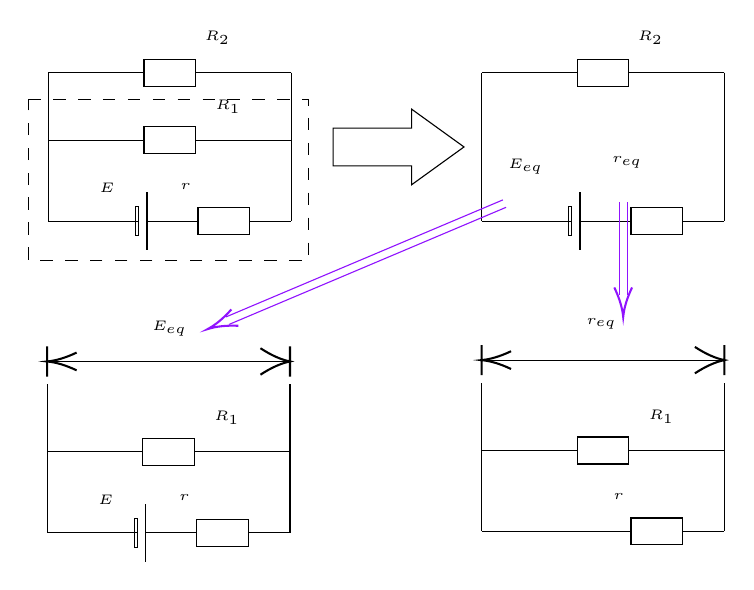
\begin{tikzpicture}[x=0.75pt,y=0.75pt,yscale=-1.3,xscale=1.3]
%uncomment if require: \path (0,300); %set diagram left start at 0, and has height of 300

%Shape: Resistor [id:dp7232411406538839] 
\draw   (245.9,100) -- (265.1,100) -- (265.1,110) -- (245.9,110) -- (245.9,100) -- cycle (240.5,105) -- (245.9,105) (265.1,105) -- (270.5,105) ;
%Shape: Battery [id:dp6693718019533714] 
\draw   (210.5,105) -- (224,105) (227,94.36) -- (227,115.64) (227,105) -- (240.5,105) (222.8,99.68) -- (224,99.68) -- (224,110.32) -- (222.8,110.32) -- (222.8,99.68) -- cycle ;
%Straight Lines [id:da16042882813115766] 
\draw    (190.5,50) -- (190.5,105) ;
%Straight Lines [id:da9402822543750411] 
\draw    (280.5,50) -- (280.5,105) ;
%Straight Lines [id:da12067780236857573] 
\draw    (190.5,105) -- (210.5,105) ;
%Straight Lines [id:da32759114986333504] 
\draw    (270.5,105) -- (280.5,105) ;
%Shape: Resistor [id:dp044708648259699446] 
\draw   (225.9,70) -- (245.1,70) -- (245.1,80) -- (225.9,80) -- (225.9,70) -- cycle (220.5,75) -- (225.9,75) (245.1,75) -- (250.5,75) ;
%Straight Lines [id:da8149590161538551] 
\draw    (220.5,75) -- (190.5,75) ;
%Straight Lines [id:da37292062821096206] 
\draw    (280.5,75) -- (250.5,75) ;
%Shape: Resistor [id:dp8915224058603441] 
\draw   (225.9,45) -- (245.1,45) -- (245.1,55) -- (225.9,55) -- (225.9,45) -- cycle (220.5,50) -- (225.9,50) (245.1,50) -- (250.5,50) ;
%Straight Lines [id:da8050738969027882] 
\draw    (220.5,50) -- (190.5,50) ;
%Straight Lines [id:da41847017454589475] 
\draw    (280.5,50) -- (250.5,50) ;
%Shape: Resistor [id:dp8946522623697388] 
\draw   (406.4,100) -- (425.6,100) -- (425.6,110) -- (406.4,110) -- (406.4,100) -- cycle (401,105) -- (406.4,105) (425.6,105) -- (431,105) ;
%Shape: Battery [id:dp4946459974897708] 
\draw   (371,105) -- (384.5,105) (387.5,94.36) -- (387.5,115.64) (387.5,105) -- (401,105) (383.3,99.68) -- (384.5,99.68) -- (384.5,110.32) -- (383.3,110.32) -- (383.3,99.68) -- cycle ;
%Straight Lines [id:da8491657091150393] 
\draw    (351,50) -- (351,105) ;
%Straight Lines [id:da8293033184283518] 
\draw    (441,50) -- (441,105) ;
%Straight Lines [id:da6903389383039646] 
\draw    (351,105) -- (371,105) ;
%Straight Lines [id:da4919692394445716] 
\draw    (431,105) -- (441,105) ;
%Shape: Resistor [id:dp9226843247374981] 
\draw   (386.4,45) -- (405.6,45) -- (405.6,55) -- (386.4,55) -- (386.4,45) -- cycle (381,50) -- (386.4,50) (405.6,50) -- (411,50) ;
%Straight Lines [id:da5240532491363821] 
\draw    (381,50) -- (351,50) ;
%Straight Lines [id:da8200773875832033] 
\draw    (441,50) -- (411,50) ;
%Right Arrow [id:dp12563132066413996] 
\draw   (296,70.5) -- (325.1,70.5) -- (325.1,63.5) -- (344.5,77.5) -- (325.1,91.5) -- (325.1,84.5) -- (296,84.5) -- cycle ;
%Shape: Rectangle [id:dp8119351522330263] 
\draw  [dash pattern={on 4.5pt off 4.5pt}] (183,60) -- (287,60) -- (287,119.5) -- (183,119.5) -- cycle ;
%Shape: Resistor [id:dp9181595801961024] 
\draw   (245.4,215.5) -- (264.6,215.5) -- (264.6,225.5) -- (245.4,225.5) -- (245.4,215.5) -- cycle (240,220.5) -- (245.4,220.5) (264.6,220.5) -- (270,220.5) ;
%Shape: Battery [id:dp8638451126944211] 
\draw   (210,220.5) -- (223.5,220.5) (226.5,209.86) -- (226.5,231.14) (226.5,220.5) -- (240,220.5) (222.3,215.18) -- (223.5,215.18) -- (223.5,225.82) -- (222.3,225.82) -- (222.3,215.18) -- cycle ;
%Straight Lines [id:da9493469917798139] 
\draw    (190,165.5) -- (190,220.5) ;
%Straight Lines [id:da9469350410050841] 
\draw    (280,165.5) -- (280,220.5) ;
%Straight Lines [id:da9707422227961422] 
\draw    (190,220.5) -- (210,220.5) ;
%Straight Lines [id:da47902505858245004] 
\draw    (270,220.5) -- (280,220.5) ;
%Shape: Resistor [id:dp44228410120226136] 
\draw   (225.4,185.5) -- (244.6,185.5) -- (244.6,195.5) -- (225.4,195.5) -- (225.4,185.5) -- cycle (220,190.5) -- (225.4,190.5) (244.6,190.5) -- (250,190.5) ;
%Straight Lines [id:da7513382191815712] 
\draw    (220,190.5) -- (190,190.5) ;
%Straight Lines [id:da4997577437287888] 
\draw    (280,190.5) -- (250,190.5) ;
%Straight Lines [id:da29586923725139136] 
\draw    (190,157) -- (280,157) ;
\draw [shift={(280,157)}, rotate = 180] [color={rgb, 255:red, 0; green, 0; blue, 0 }  ][line width=0.75]    (0,5.59) -- (0,-5.59)(10.93,-4.9) .. controls (6.95,-2.3) and (3.31,-0.67) .. (0,0) .. controls (3.31,0.67) and (6.95,2.3) .. (10.93,4.9)   ;
\draw [shift={(190,157)}, rotate = 0] [color={rgb, 255:red, 0; green, 0; blue, 0 }  ][line width=0.75]    (0,5.59) -- (0,-5.59)(10.93,-3.29) .. controls (6.95,-1.4) and (3.31,-0.3) .. (0,0) .. controls (3.31,0.3) and (6.95,1.4) .. (10.93,3.29)   ;
%Shape: Resistor [id:dp0668394417226108] 
\draw   (406.4,215) -- (425.6,215) -- (425.6,225) -- (406.4,225) -- (406.4,215) -- cycle (401,220) -- (406.4,220) (425.6,220) -- (431,220) ;
%Straight Lines [id:da585027680617425] 
\draw    (351,165) -- (351,220) ;
%Straight Lines [id:da24202593084033786] 
\draw    (441,165) -- (441,220) ;
%Straight Lines [id:da7950606810490672] 
\draw    (351,220) -- (401,220) ;
%Straight Lines [id:da9338085769888853] 
\draw    (431,220) -- (441,220) ;
%Shape: Resistor [id:dp9351098294796791] 
\draw   (386.4,185) -- (405.6,185) -- (405.6,195) -- (386.4,195) -- (386.4,185) -- cycle (381,190) -- (386.4,190) (405.6,190) -- (411,190) ;
%Straight Lines [id:da7426770619592475] 
\draw    (381,190) -- (351,190) ;
%Straight Lines [id:da4939519386694273] 
\draw    (441,190) -- (411,190) ;
%Straight Lines [id:da5374904022522706] 
\draw    (351,156.5) -- (441,156.5) ;
\draw [shift={(441,156.5)}, rotate = 180] [color={rgb, 255:red, 0; green, 0; blue, 0 }  ][line width=0.75]    (0,5.59) -- (0,-5.59)(10.93,-4.9) .. controls (6.95,-2.3) and (3.31,-0.67) .. (0,0) .. controls (3.31,0.67) and (6.95,2.3) .. (10.93,4.9)   ;
\draw [shift={(351,156.5)}, rotate = 0] [color={rgb, 255:red, 0; green, 0; blue, 0 }  ][line width=0.75]    (0,5.59) -- (0,-5.59)(10.93,-3.29) .. controls (6.95,-1.4) and (3.31,-0.3) .. (0,0) .. controls (3.31,0.3) and (6.95,1.4) .. (10.93,3.29)   ;
%Straight Lines [id:da48480372543600314] 
\draw [color={rgb, 255:red, 144; green, 19; blue, 254 }  ,draw opacity=1 ]   (360.08,99.88) -- (257.45,143.27)(358.92,97.12) -- (256.28,140.5) ;
\draw [shift={(249.5,145)}, rotate = 337.08] [color={rgb, 255:red, 144; green, 19; blue, 254 }  ,draw opacity=1 ][line width=0.75]    (10.93,-3.29) .. controls (6.95,-1.4) and (3.31,-0.3) .. (0,0) .. controls (3.31,0.3) and (6.95,1.4) .. (10.93,3.29)   ;
%Straight Lines [id:da6108098931367383] 
\draw [color={rgb, 255:red, 144; green, 19; blue, 254 }  ,draw opacity=1 ]   (405,98) -- (405,132.5)(402,98) -- (402,132.5) ;
\draw [shift={(403.5,140.5)}, rotate = 270] [color={rgb, 255:red, 144; green, 19; blue, 254 }  ,draw opacity=1 ][line width=0.75]    (10.93,-3.29) .. controls (6.95,-1.4) and (3.31,-0.3) .. (0,0) .. controls (3.31,0.3) and (6.95,1.4) .. (10.93,3.29)   ;

% Text Node
\draw (212.5,88.5) node [anchor=north west][inner sep=0.75pt]   [align=left] {$ $};
% Text Node
\draw (208.5,90) node [anchor=north west][inner sep=0.75pt]  [font=\tiny] [align=left] {$\displaystyle \ms E$};
% Text Node
\draw (238.5,90) node [anchor=north west][inner sep=0.75pt]  [font=\tiny] [align=left] {$\displaystyle r$};
% Text Node
\draw (251.5,59) node [anchor=north west][inner sep=0.75pt]  [font=\tiny] [align=left] {$\displaystyle R_{1}$};
% Text Node
\draw (247.5,33.5) node [anchor=north west][inner sep=0.75pt]  [font=\tiny] [align=left] {$\displaystyle R_{2}$};
% Text Node
\draw (373,88.5) node [anchor=north west][inner sep=0.75pt]   [align=left] {$ $};
% Text Node
\draw (360,81) node [anchor=north west][inner sep=0.75pt]  [font=\tiny] [align=left] {$\displaystyle \ms E_{eq}$};
% Text Node
\draw (398.5,80) node [anchor=north west][inner sep=0.75pt]  [font=\tiny] [align=left] {$\displaystyle r_{eq}$};
% Text Node
\draw (408,33.5) node [anchor=north west][inner sep=0.75pt]  [font=\tiny] [align=left] {$\displaystyle R_{2}$};
% Text Node
\draw (212,204) node [anchor=north west][inner sep=0.75pt]   [align=left] {$ $};
% Text Node
\draw (208,205.5) node [anchor=north west][inner sep=0.75pt]  [font=\tiny] [align=left] {$\displaystyle \ms E$};
% Text Node
\draw (238,205.5) node [anchor=north west][inner sep=0.75pt]  [font=\tiny] [align=left] {$\displaystyle r$};
% Text Node
\draw (251,174.5) node [anchor=north west][inner sep=0.75pt]  [font=\tiny] [align=left] {$\displaystyle R_{1}$};
% Text Node
\draw (228,141) node [anchor=north west][inner sep=0.75pt]  [font=\tiny] [align=left] {$\displaystyle \ms E_{eq}$};
% Text Node
\draw (399,205) node [anchor=north west][inner sep=0.75pt]  [font=\tiny] [align=left] {$\displaystyle r$};
% Text Node
\draw (412,174) node [anchor=north west][inner sep=0.75pt]  [font=\tiny] [align=left] {$\displaystyle R_{1}$};
% Text Node
\draw (389,140) node [anchor=north west][inner sep=0.75pt]  [font=\tiny] [align=left] {$\displaystyle r_{eq}$};


\end{tikzpicture}

\end{center}